\documentclass[a4paper,12pt]{article} % тип документа

%  Русский язык
\usepackage{multirow}
\usepackage{wrapfig}
\usepackage[T2A]{fontenc}			% кодировка
\usepackage[utf8]{inputenc}			% кодировка исходного текста
\usepackage[english,russian]{babel}	% локализация и переносы

\usepackage{indentfirst} %Красная строка
\usepackage[a4paper,top=1.3cm,bottom=2cm,left=1.5cm,right=1.5cm,marginparwidth=0.75cm]{geometry}
\usepackage[usenames]{color}
\usepackage{colortbl}
\usepackage{float}

\usepackage{graphicx}%картинки
\usepackage{wrapfig}%обтекание текстом теблиц и картинок
%гиперссылки
\usepackage{hyperref}
\usepackage[rgb]{xcolor}
\hypersetup{     %гипперсылки
 colorlinks=true, %false:ссылки в рамках
 urlcolor=blue   %на URL
 }
% Заметки
\usepackage{todonotes}

% Математика
\usepackage{amsmath,amsfonts,amssymb,amsthm,mathtools} 
\usepackage{hyperref}

\begin{document}

\begin{titlepage}
\begin{center}
    {\large МОСКОВСКИЙ ФИЗИКО-ТЕХНИЧЕСКИЙ ИНСТИТУТ (НАЦИОНАЛЬНЫЙ ИССЛЕДОВАТЕЛЬСКИЙ УНИВЕРСИТЕТ)}
\end{center}
\begin{center}
    {\largeФизтех-школа физики и исследований им. Ландау}
\end{center}

\vspace{3.5cm}

\begin{center}
    
\includegraphics[width=0.4\linewidth]{hv_full.png}
\end{center}
\vspace{0.1cm}
{\huge
\begin{center}
    {\bf Лабораторная работа 1.3.2}\\
    Определение модуля кручения
\end{center}
}
\vspace{2cm}
\begin{flushright}
{\LARGE Авторы:\\ Петров Олег \\
\vspace{0.2cm}
Б02-202}
\end{flushright}
\vspace{3.5cm}
\begin{center}
    Долгопрудный 2022
\end{center}
\end{titlepage}

\section{Aннотация}
\textbf{Цель работы:}измерение углов закручивания в зависимости от приложенного момента
сил, определение модулей для проволки по измерениям периодов крутильных колебаний подвешенного на
ней маятника\\
\textbf{Оборудование:}проволка из исследуемого материала,
грузы, секундомер, микрометр, рулетка, линйка.
\section{Теоретические сведения}
При закручивании цилиндрических стержней круглого сечения распределение деформаций
 и напряжений одинаково по длине стержня только вдали от мест, где прикладываются закручивающие моменты.
Для этих областей можно считать, что каждое поперечное сечение поворачивается поворачивается как жествкое,
то есть частички материала не сходят с радиальных линий, на которых они были в начале, и все
эти линии поворачиваются на один и тот же угол. Такое напряженное состояние назвается чистым кручением.\\

При такой деформации любая прямая линия, проведенная до закручивания цилиндра почастицам материала и параллельная оси симметрии,
при закручивании превращается в спираль(винтовую линию). \\

Покажем, что касательное напряжение напряжение в поперечном сечении увеличивается пропорцианально
 расстоянию до оси вращения.
Рассмотрим в цилиндре колечко бесконечно малой толщиной $dr$ и высоты $dl$. При закручивании верхнее колечко поворачивается относительно 
нижнего на угол $d\varphi$, а образующая наклоняется на угол $\alpha$. Тогда при малы углах справедливо соотношение:
\begin{equation}
    \alpha dl= r d\varphi 
\end{equation}

Касательное наряжение $\tau $ связано с углом $\alpha$ линейной зависимостью через модуль сдвига $G$,
 и следовательно растет с увеличением расстоянием от оси:
\begin{equation}
    \tau = G\cdot \alpha =Gr\frac{d\varphi}{dl} 
\end{equation}

Эти касательные напряжения создают момент сил относительно оси цилиндра:

\begin{equation}
    dM=2\pi r dr \cdot r\cdot \tau  
\end{equation}

Интегрируя это выражение по всем колечкам от оси цилиндра до его радиуса R находим суммарный
момент сил:
\begin{equation}
    M = \frac{\pi G R^{4}}{2} \frac{d \varphi }{d l} 
\end{equation}

Так как момент сил не меняется по длине цилиндра. Тогда для связи приложенного
момента сил $M$ и угла поворота $\varphi$ поперечных сечений цилиндра имеем:
\begin{equation}
    M=\frac{\pi R^{4}G}{2l}\varphi=f \varphi
\end{equation}
Где $f$ - модуль кручения связанный с модулем сдвига $G$ соотношением:
\begin{equation}
    G=\frac{2l}{\pi R^{4}}f
\end{equation}

%\section{Определение модуля кручения стержня статистическим методом}
%\subsection{Экспериментальная установка}
%
%\subsection{Результаты эксперимента и обраюотка данных}
%\begin{itemize}
%    \item Установим зрительную трубку так, чтобы в нее было четко видно отражение
%от шкалы в зеркальце. Установим параметры системы:
%$$l= \ \text{}, D= \ \text{},d= \ \text{}, g = 9.8155 \pm 0.0005 \ \text{м}c^{-2} $$
%где l -  расстояние до шкалы, D - диаметр диска, d - диаметр стержня.
%    \item Увеличиваем нагрузку на нити с помощью набора грузов. Проводим серию измерений при
%увелечении и уменьшении массы грузов. Полученные данные заносим в таблицу. Расчет угла $\varphi$
%и момента сил производим по формулам:
%$$M=D P = D m g, \ \ \ \varphi = \arctg (\Delta l/2l)  $$
%
%\item По полученным данным строим график зависимости
%\end{itemize}
В системе можно возбудить крутильные колебания. Вращение стержня с закрепленными
на нем грузиками вокрунг вертикальной оси проиходит под действием упругого момента $M$.
С учетом выражения для момента $M$ получим, что это вращение описывается уравнением колебаний:
\begin{equation}
    I\frac{d^2 \varphi }{d t^2} + f \varphi =0
\end{equation}
Следовательно период кoлебаний системы связан с расстоянием $r$ от оси вращения до грузов и
моментом инерции стержня $I_0$ следующим образом:
\begin{equation}
    T^2=(2\pi)^2\frac{I}{f}=(2\pi)^2\frac{I_0}{f}+(2\pi)^2\frac{(m_1+m_2)}{f}r^2
\end{equation}
Эти зависимости были получены для незатухающих колебаний. Поэтому для их применения необходимо убедиться,
что в рассматриваемой системе диссипативными силами можно пренебречь. Для этого стоит убедиться, что период колебаний
не зависит от начальной амплитуды и что амплитуда уменшьется не более чем в 2 раза после около 10 колебаний.
\section{Экспериментальная установка}

Экспериментальная установка, используемая в этой части работы,
изображена на рис. 1 и состоит из длинной вертикально висящей право-
локи П, к нижнему концу которой прикреплен горизонтальный метал-
лический стержень С с двумя симметрично расположенными грузами
Г. Их положение на стержне можно фиксировать. Верхний конец право-
локи зажать в цангу и при помощи специального приспособления может
вместе с цангой поворачиваться вокруг вертикальной оси. Таким спо-
собом в системе можно возбуждать крутильные колебания. Вращение
стержня С с закрепленными на нем грузами Г вокруг вертикальной
оси происходит под действием упругого момента, возникающего в проволоке.

\begin{figure}[!h]
    \begin{center}
        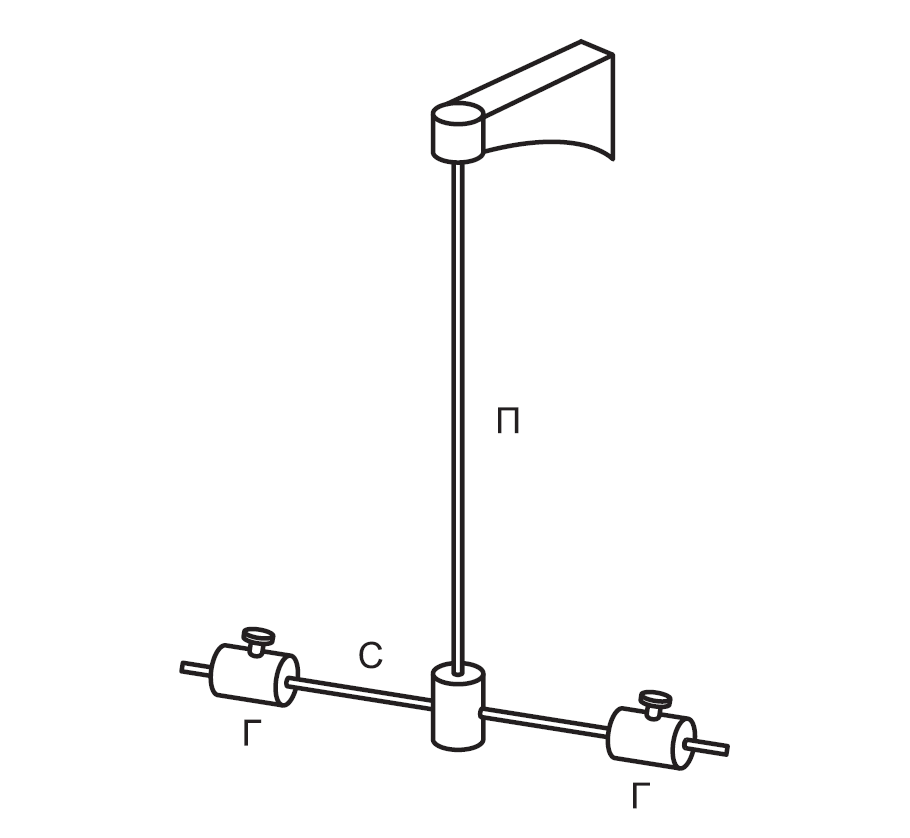
\includegraphics[scale=0.7]{ystanovka.png}
        \begin{center}
        \caption{Схема установки}
        \end{center}
        \label{graphic1b}
    \end{center}
\end{figure}

\section{Результаты эксперимента и обработка данных}

\begin{itemize}
    \item Перед началом работы установим параметры системы:
$$l=174 \pm 1 \ \text{см},\ \ \ d = 1.98 \pm 0.01 \ \text{мм}, \ \ \ m_1=377.5 \pm 0.05 \ \text{гр}, \ \ \ m_2= 373.1 \pm 0.05 \ \text{гр} $$
$$\varepsilon_{l}=0.5 \%, \ \ \ \varepsilon_{d}= 0.5 \%,\ \ \ \varepsilon_{m_1}=0.01 \%,\ \ \ \varepsilon_{m_2}= 0.01\%,$$
    \item Укрепим грузы на некотором одинаковом расстоянии от оси и возбудим в системе крутильныйколебания. Перед 
началом измерений убедимся, что мы выбрали правильный диапозон амплитуд для измерений,
в котором можно пренебречь затуханием и применять уравнения гармонических колебаний. Для 
этого убедимся в том, что амплитуда колебаний уменьшается не более чем в 2 раза после 10-15 периодов
колебаний.
    \item Убедившись в том, что затуханием можно пренебречь установим, грузы на стержне на одинаковом расстоянии от оси $r$
от оси симметрии системы до центра масс каждого из грузов. Будем измерять период колебаний $T$ в зависимости
от длины $r$ и заносим данные в таблицу ниже:
\begin{table}[!ht]
    \centering
    \begin{tabular}{llllll}\hline
        $t$,с&$N$&$T$,с&$l$,см&$l^2,\ \text{см}^2$&$T^2,\ \text{с}^2$\\ \hline
        72.04 & 23 & 3.13 & 100 & 10000 & 9.81  \\ 
        37.78 & 12 & 3.15 & 100 & 10000 & 9.91  \\ \hline
        57.65 & 20 & 2.88 & 90 & 8100 & 8.31  \\ 
        57.66 & 20 & 2.88 & 90 & 8100 & 8.31  \\ 
        106.74 & 37 & 2.88 & 90 & 8100 & 8.32  \\ 
        54.84 & 19 & 2.89 & 90 & 8100 & 8.33  \\ 
        57.88 & 20 & 2.89 & 90 & 8100 & 8.38  \\ \hline
        79.01 & 30 & 2.63 & 80 & 6400 & 6.94  \\ 
        55.16 & 21 & 2.63 & 80 & 6400 & 6.90  \\ \hline
        50 & 21 & 2.38 & 70 & 4900 & 5.67  \\ \hline
        45.09 & 21 & 2.15 & 60 & 3600 & 4.61  \\ \hline
        48.45 & 25 & 1.94 & 50 & 2500 & 3.76  \\
        46.16 & 24 & 1.92 & 50 & 2500 & 3.70  \\ \hline
    \end{tabular}
    \caption{измерение периода в зависимости от длины плеча}
\end{table}
    \item По полученным данным строим график зависимости $r^2$ от $T^2$ пользуясь
 методом наименьших квадратов (МНК). По величине наклона определяем модуль кручения и его погрешность.

\begin{figure}[!h]
    \begin{center}
        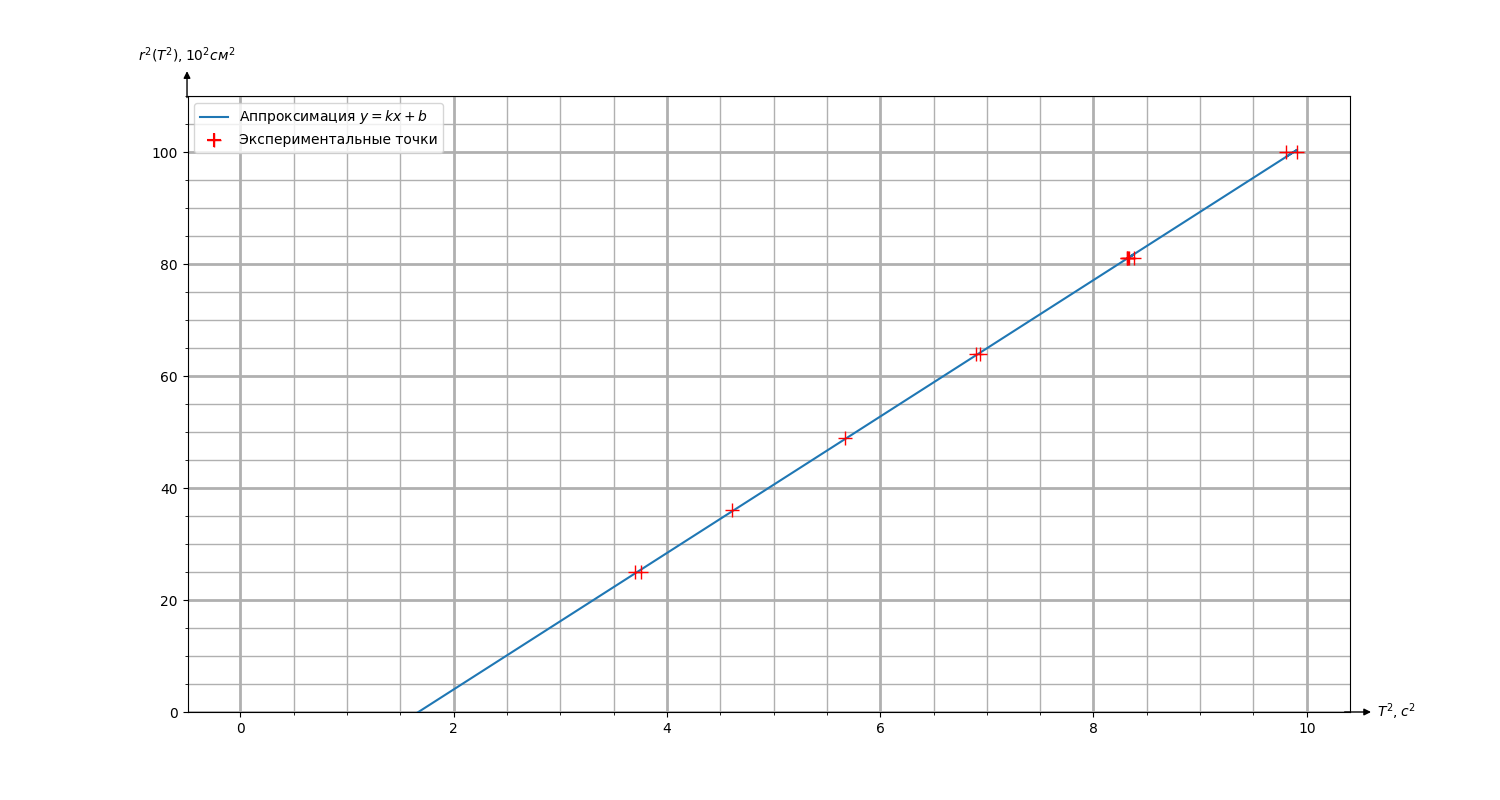
\includegraphics[width=1\textwidth]{graphic}
        \begin{center}
        \caption{График зависимости $r^2$ от $T^2$}
        \end{center}
        \label{graphic1b}
    \end{center}
\end{figure}

Определим коэффицент наклона графика и его случайную погрешность пользуясь формулами МНК и ковариацией
 $D_{x,y}=\langle x y \rangle - \langle x \rangle  \langle y\rangle $:
$$k=\dfrac{\langle T^2 r^2 \rangle-\langle T^2 \rangle \langle r^2 \rangle}{\langle T^4 \rangle - \langle T^2\rangle^2}= \dfrac{D_{r^2 \cdot T^2}}{D_{T^2 \cdot T^2}} = 12.18 \cdot \text{м}^2/\text{c}^2$$ %\ \text{$\dfrac{\text{м}^2}{\text{c}^2}$} $$
$$\varepsilon_k^\text{случ}=\frac{1}{k\sqrt{N-2}}\sqrt{\frac{\langle r^4 \rangle - \langle r^2 \rangle^2}{\langle T^4 \rangle - \langle T^2 \rangle^2} - k^2 }= 0.5\%,\ \ \ 
\varepsilon_k^\text{сист}=2\sqrt{\varepsilon^2_{T}+\varepsilon^2_{r}}=0.6 \%$$
$$\varepsilon_k=\sqrt{\varepsilon_\text{сист}^2+\varepsilon_\text{случ}^2} = 0.7 \%$$
По итогу получаем значение коэффицента наклона прямой: $k=12.18 \pm 0.08 \ \text{м}^2/\text{c}^2$. При подсчете погрешности $f$ учтем, что $\varepsilon_{m} \ll \varepsilon_{k}$.
Теперь мы можем получить значение для модуля кручения пользуясь формулами:
$$f=(2\pi)^2(m_1+m_2)\cdot k = 3.6 \cdot 10^{-2} \ \text{Нм}, \ \ \  \varepsilon_{f} \approx \varepsilon_{k} = 0.7 \%$$
Для итогового значения модуля кручения имеем: $f=3.61 \pm 0.02 \ 10^{-2} \ \text{Нм}$ 
    \item Теперь зная геометрические параметры проволки по найденному модулю кручения $f$ мы можем найти модуль
сдвига $G$ пользуясь формулой:
$$G=\frac{32l}{\pi d^{4}}f = 40.8 \ \text{Гпа} \ \ \ \varepsilon_{G}=\sqrt{\varepsilon^2_{f}+\varepsilon^2_{l}+16\varepsilon^2_{d}} = 2\%$$
Получаем итоговое значение для модуля сдвига: $G= 40.8 \pm 0.8$ Гпа.
\end{itemize}


\section{Выводы}
В результате эксперимента были получены значения для модуля кручения $f=3.61 \pm 0.02 \ 10^{-2} \ \text{Нм}$ проволки и
модуля сдвига проволки $G= 40.8 \pm 0.8 $ Гпа с приемлемой точностью $\varepsilon_{G} = 2\%$. Можно также заметить, что модуль сдвига
материала проволки в пределах погрешности совпадает с модулем сдвига сплавов меди в первую очередь и во вторую очередь частично попадает
 в значений модулей сдвига следующих материалов: титан, бронза, чугун, нейзильбер.

\end{document}